\documentclass[11pt,a4paper]{article}
\usepackage[margin=25mm]{geometry}
\usepackage{graphicx,booktabs,amsmath,hyperref}
\hypersetup{colorlinks=true,linkcolor=blue,urlcolor=blue}
\title{Molecular prioritization of layered-perovskite spacers from device literature}
\author{Research working manuscript}
\date{19 October 2026}
\begin{document}\maketitle
\begin{abstract}
We reconstructed 749 reported solar-cell devices across 134 publications and 42 source-verified ionic spacer structures (31 monovalent).
A DOI-cross-fitted context model generates chemistry-level PCE residual labels in each outer training fold. 
Fixed models and chance baselines are evaluated with chemistry holdouts and leave-one-family-out testing.
For monovalent chemistry, the exploratory nested AP of logistic2 is 0.420 versus 0.285 for random ranking. Model choice was informed by these same external comparisons, so this is not a selection-independent estimate.
Out of 13595 PubChem records, 2087 distinct screened monovalent precursor ions were considered; ten molecules were selected for controlled fabrication.
\end{abstract}
\section{Introduction}
Organic spacer cations affect the processing and properties of layered halide perovskites. 
Existing literature offers many device records but few chemically independent spacer identities. 
Our aim is to determine whether those records support reliable decisions on which untested cations to examine. 
The analysis treats spacers as the prediction units and records published processing conditions as context.
\section{Data and chemical representation}
The source contains 792 device records; 749 satisfy single verified spacer requirements.
Original charged species, including aromatic and diammonium ions, are retained as defined by the source chemical registry.
The 35 ordered RDKit descriptors are generated anew for each ion. 
A separate amine-site transformation supplies monovalent candidate structures from neutral PubChem precursors.
\section{Validation design}
The device-context estimator is a standardized ridge regression with alpha 10. DOI-grouped out-of-fold residuals define spacer median uplift.
Within each outer chemistry fold, both the context model and the upper-quintile label threshold are regenerated using training chemistry only.
We report ten repetitions of five-fold stratified chemistry holdout and leave-one-molecular-family-out validation.
The candidate ranker is frozen to two-descriptor logistic regression after exploratory inspection of outer validation scores. The AP values in this paper are exploratory model-comparison statistics; an unbiased post-selection assessment requires genuinely external prospective data.
The candidate ranking models are fixed logistic regression with 2 or 35 descriptors and a fixed XGBoost ranker, alongside constant-score and random-order baselines.
\section{Results}
\begin{table}[h]\centering
\caption{Pooled average precision (AP) for held-out spacer identities.}
\begin{tabular}{lrrrr}\toprule
Model & All nested & All family & Mono nested & Mono family\\ \midrule
Random ordering & 0.294 & 0.290 & 0.285 & 0.292\\
Constant score & 0.236 & 0.199 & 0.225 & 0.247\\
Logistic (2) & 0.482 & 0.533 & 0.420 & 0.462\\
Logistic (35) & 0.576 & 0.798 & 0.449 & 0.398\\
XGBoost (35) & 0.484 & 0.506 & 0.412 & 0.431\\
\bottomrule\end{tabular}\end{table}
\section{Literature-source and family diagnostics}
Of 7 positive monovalent cations in full-data labels, 5 have only one supporting DOI. Removing their only publication removes the target observation, rather than providing an independent validation of positive status.
For supported multisource cations, the full-context model and upper-quintile threshold are recalculated after deleting individual publications. The accompanying source-stability table records label changes and cases in which no evidence remains.
Only 2 of 8 monovalent held-out molecular families contain both positive and negative labels under fold-specific context refitting. Scores originate from different family-exclusion fits; pooled AP includes between-family ordering and is not equivalent to within-family ranking quality.
A publication-disjoint diagnostic removes every publication containing a held-out spacer from the corresponding training devices before context fitting. 13 source-disjoint folds were evaluable. This stress test changes available training chemistry and source support; it is reported alongside, rather than substituted for, the original model comparison.
\begin{figure}[h]\centering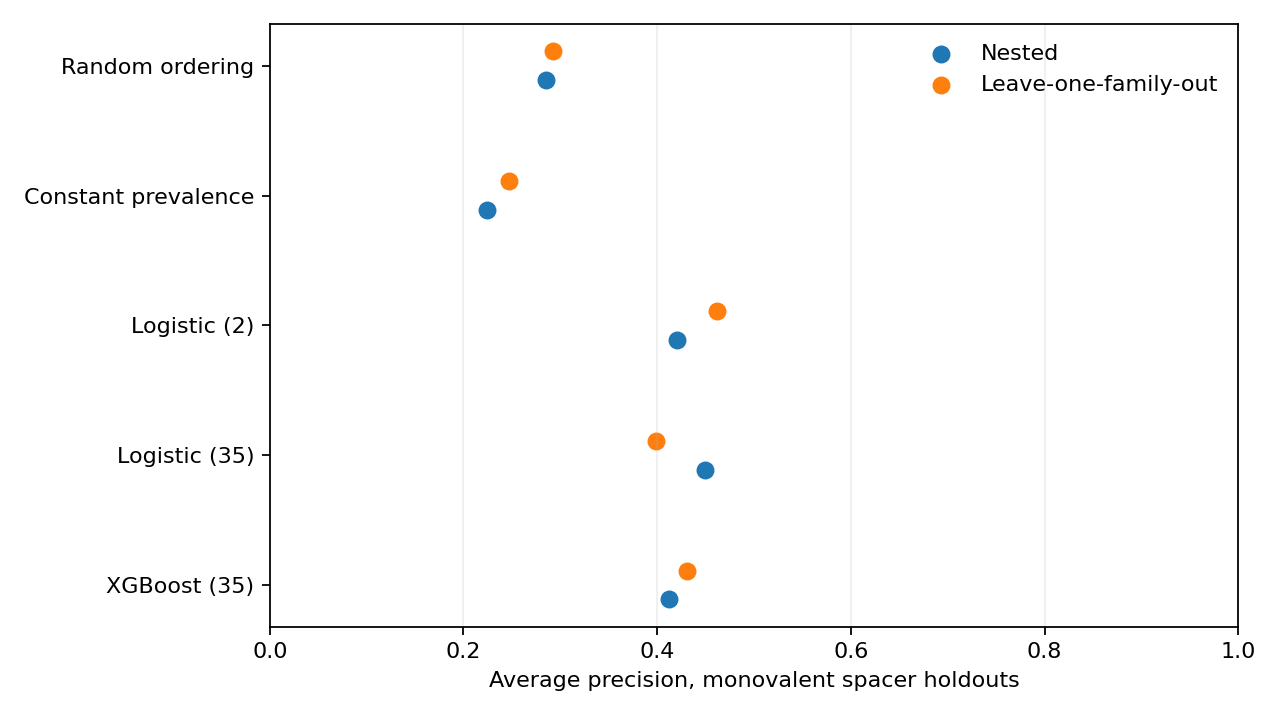
\includegraphics[width=.89\linewidth]{evaluation.png}
\caption{Fixed models under monovalent chemistry and family holdout protocols.}\end{figure}
\section{Molecular screening}
The chemical filter retains 3296 unique candidate ions, including 2087 monovalent and 1209 non-monovalent structures.
The frozen screening model is logistic2. The shared score and domain gates yield 121 candidates, followed by 74 Pareto-optimal entries and ten diversity-selected molecules.
All ten shortlist molecules are in the moderate extrapolation category under the current empirical fingerprint and descriptor criteria. This class has not been calibrated to an expected prediction error.
The model score is an uncalibrated mean classifier output, not the probability of successful device fabrication. Candidate priority combines rank, uncertainty, synthetic accessibility, applicability and novelty. Final rank is the order of diversity selection and need not follow descending model score.
\begin{figure}[h]\centering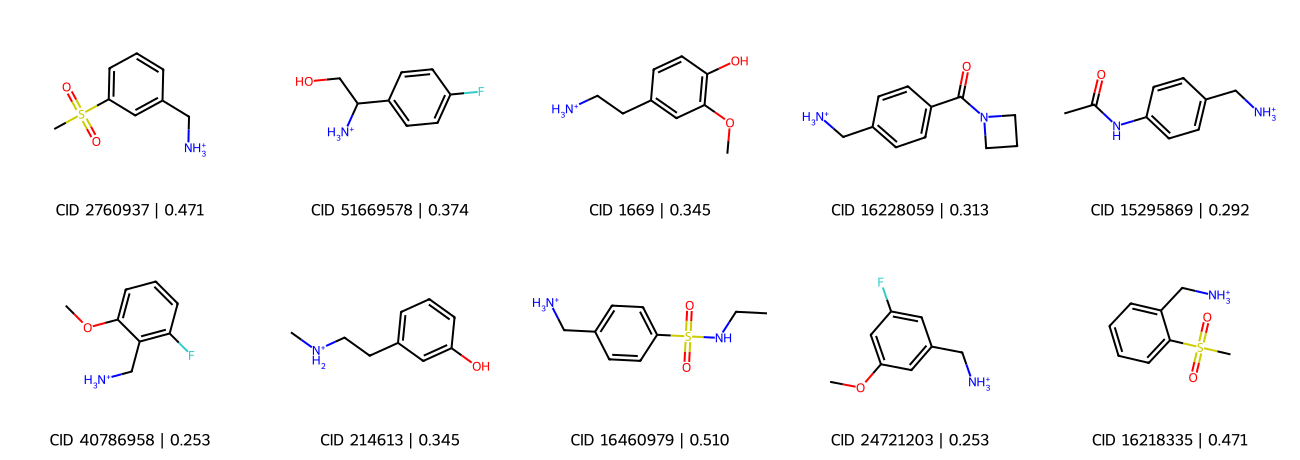
\includegraphics[width=\linewidth]{candidate_structures.png}
\caption{Ten current monovalent candidate cations. Scores are retrospective model rankings.}\end{figure}
\section{Experimental test}
We propose 12 prespecified new spacer compounds: four high-ranked, four chemistry-matched lower-ranked, and four random eligible choices.
Two known spacers serve as batch references. The primary PCE endpoint is evaluated across independent fabrication batches with the spacer, not device, as the independent ranking unit.
Prospective devices supply the first model-selection-independent comparison of the frozen two-descriptor ranker with random ordering and prespecified chemical baselines.
Diffraction, PL/TRPL and morphology measurements provide secondary mechanistic evidence.
\section{Data and computation}
The complete clean analysis is regenerated from source-verified device matrices, chemical registries and the PubChem query pool. 
Code and data-file digests, feature order, package versions and model configuration are recorded in the accompanying manifest.
\end{document}
